\documentclass[ignorenonframetext,]{beamer}
\setbeamertemplate{caption}[numbered]
\setbeamertemplate{caption label separator}{: }
\setbeamercolor{caption name}{fg=normal text.fg}
\beamertemplatenavigationsymbolsempty
\usepackage{lmodern}
\usepackage{amssymb,amsmath}
\usepackage{ifxetex,ifluatex}
\usepackage{fixltx2e} % provides \textsubscript
\ifnum 0\ifxetex 1\fi\ifluatex 1\fi=0 % if pdftex
  \usepackage[T1]{fontenc}
  \usepackage[utf8]{inputenc}
\else % if luatex or xelatex
  \ifxetex
    \usepackage{mathspec}
  \else
    \usepackage{fontspec}
  \fi
  \defaultfontfeatures{Ligatures=TeX,Scale=MatchLowercase}
\fi
\usetheme{AnnArbor}
\usecolortheme{dolphin}
\usefonttheme{professionalfonts}
% use upquote if available, for straight quotes in verbatim environments
\IfFileExists{upquote.sty}{\usepackage{upquote}}{}
% use microtype if available
\IfFileExists{microtype.sty}{%
\usepackage{microtype}
\UseMicrotypeSet[protrusion]{basicmath} % disable protrusion for tt fonts
}{}
\newif\ifbibliography
\usepackage{longtable,booktabs}
\usepackage{caption}
% These lines are needed to make table captions work with longtable:
\makeatletter
\def\fnum@table{\tablename~\thetable}
\makeatother
\usepackage{graphicx,grffile}
\makeatletter
\def\maxwidth{\ifdim\Gin@nat@width>\linewidth\linewidth\else\Gin@nat@width\fi}
\def\maxheight{\ifdim\Gin@nat@height>\textheight0.8\textheight\else\Gin@nat@height\fi}
\makeatother
% Scale images if necessary, so that they will not overflow the page
% margins by default, and it is still possible to overwrite the defaults
% using explicit options in \includegraphics[width, height, ...]{}
\setkeys{Gin}{width=\maxwidth,height=\maxheight,keepaspectratio}

% Prevent slide breaks in the middle of a paragraph:
\widowpenalties 1 10000
\raggedbottom

\AtBeginPart{
  \let\insertpartnumber\relax
  \let\partname\relax
  \frame{\partpage}
}
\AtBeginSection{
  \ifbibliography
  \else
    \let\insertsectionnumber\relax
    \let\sectionname\relax
    \frame{\sectionpage}
  \fi
}
\AtBeginSubsection{
  \let\insertsubsectionnumber\relax
  \let\subsectionname\relax
  \frame{\subsectionpage}
}

\setlength{\emergencystretch}{3em}  % prevent overfull lines
\providecommand{\tightlist}{%
  \setlength{\itemsep}{0pt}\setlength{\parskip}{0pt}}
\setcounter{secnumdepth}{0}


% \pgfdeclareimage[width=1cm]{logo}{./figures/monkeyTypewriter.png}
%\logo{\pgfuseimage{logo}}

\institute{University of Virginia}
\definecolor{links}{RGB}{42, 27, 129}
\definecolor{mypink2}{RGB}{219, 48, 122}
%\hypersetup{colorlinks,linkcolor=links,urlcolor=mypink2}
\usefonttheme{professionalfonts}

% \setbeamerfont{note page}{family*=pplx,size=\footnotesize} % Palatino for notes

\setbeamerfont{subtitle}{size=\small}

\definecolor{uvablue}{RGB}{0,85,150}
\definecolor{uvalibraryorange}{RGB}{252,175,23}
\definecolor{uvacream}{RGB}{241,229,199}
\definecolor{uvalightblue}{RGB}{163,220,230}

\setbeamercolor{block body}{bg=green,fg=green}
\setbeamercolor{block body alerted}{bg=green,fg=green}
\setbeamercolor{block body example}{bg=green,fg=green}

\setbeamercolor{caption name}{fg=uvablue}

\setbeamercolor{headline}{fg=uvacream,bg=uvacream}
\setbeamercolor{section}{fg=uvalibraryorange,bg=uvablue}
\setbeamercolor{frametitle}{fg=uvalibraryorange,bg=uvablue}
\setbeamercolor{palette primary}{bg=uvalibraryorange,fg=uvablue}
\setbeamercolor{palette secondary}{bg=uvablue,fg=uvablue}
\setbeamercolor{palette tertiary}{bg=uvalibraryorange,fg=uvablue}
\setbeamercolor{palette quarternary}{fg=uvalibraryorange,bg=uvablue}
\setbeamercolor{palette sidebar primary}{bg=uvalibraryorange,fg=uvablue}
\setbeamercolor{palette sidebar secondary}{fg=uvablue,bg=uvablue}
\setbeamercolor{palette sidebar tertiary}{fg=uvalibraryorange,bg=uvablue}
\setbeamercolor{palette sidebar quarternary}{fg=uvalibraryorange,bg=uvablue}
\setbeamercolor{structure}{bg=uvablue}



\useinnertheme{rectangles}

\titlegraphic{\vspace{-7.5mm}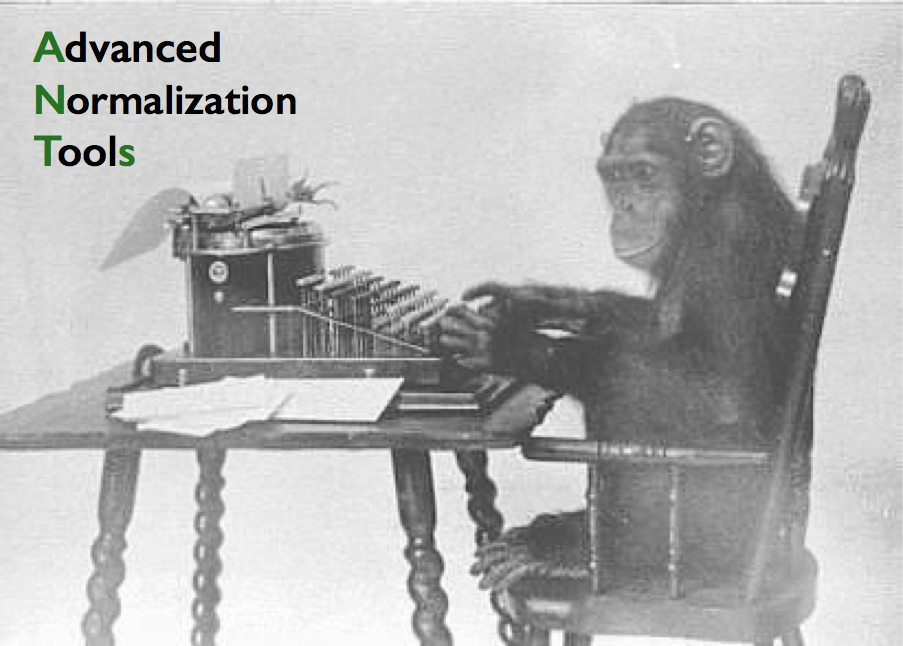
\includegraphics[width=0.45\paperwidth]{./figures/monkeyTypewriter.png}}

\title{``Dr.~Tustison (UVA) presentation''}
\author{Nick Tustison}
\date{}

\begin{document}
\frame{\titlepage}

\section{Developers and
collaborators}\label{developers-and-collaborators}

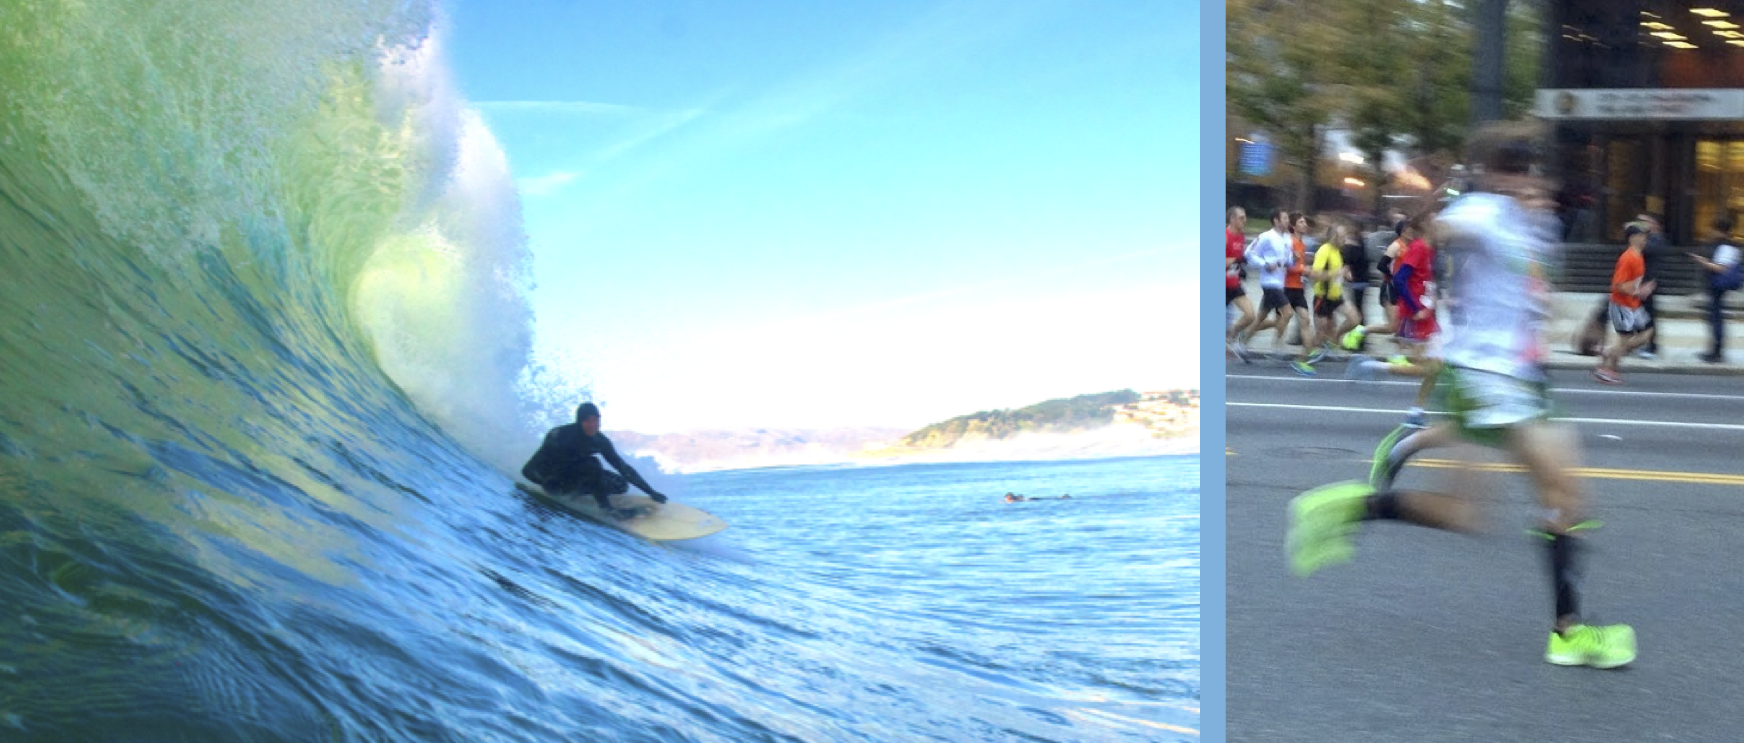
\includegraphics{./figures/brian_and_nick.png}

\begin{frame}

\includegraphics{./figures/antsCollaborators2.png}

\end{frame}

\section{Why would you care?}\label{why-would-you-care}

\begin{frame}{Software for medical image analysis}

\begin{itemize}
\item
  \href{http://fsl.fmrib.ox.ac.uk/fsldownloads/}{FSL}
\item
  \href{http://www.fil.ion.ucl.ac.uk/spm/software/}{SPM}
\item
  \href{http://www.fil.ion.ucl.ac.uk/spm/software/}{FreeSurfer}
\item
  \href{http://mipav.cit.nih.gov}{MIPAV}
\item
  \href{https://afni.nimh.nih.gov/afni}{AFNI}
\item
  Slicer, Elastix, SimpleITK, ANTs \(\longleftrightarrow\)
  \href{http://www.itk.org}{Insight Toolkit}
\item
  Many more at \href{http://idoimaging.com}{idoimaging.com}
\end{itemize}

\end{frame}

\begin{frame}{International competitions}

\begin{itemize}
\item
  \href{http://www.ncbi.nlm.nih.gov/pubmed/19195496}{Klein 2009}: MRI
  brain registration
\item
  \href{http://empire10.isi.uu.nl}{EMPIRE 2010}: CT lung registration
\item
  \href{https://masi.vuse.vanderbilt.edu/workshop2012/index.php/Main_Page}{Multi-Atlas
  Label Challenge 2012}: MRI brain registration and segmentation
\item
  \href{https://masi.vuse.vanderbilt.edu/workshop2013/index.php/MICCAI_2013_SATA_Challenge_and_Workshop:Current_events}{SATA
  Challenge 2013}: MRI cardiac and canine hind leg registration
\item
  \href{http://martinos.org/qtim/miccai2013/}{BRATS 2013}: Multi-modal
  MRI brain segmentation
\item
  \href{http://www.cardiacatlas.org/web/stacom2014/moco-introduction}{STACOM
  2014 MoCo Challenge}: MRI cardiac motion estimation
\end{itemize}

\end{frame}

\section{Major ANTs utilities}\label{major-ants-utilities}

\begin{frame}{Donoho?}

 \emph{``Papers are just advertisements for the science.''}

\end{frame}

\begin{frame}{Beyond original SyN}

\small

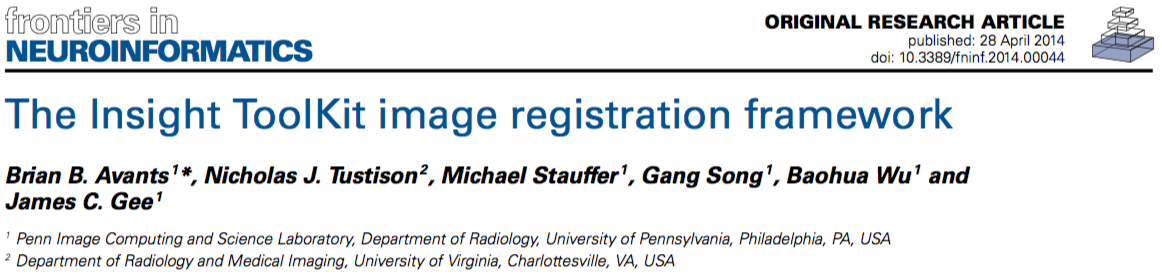
\includegraphics{./papers/figures/Frontiers_ITK.png}

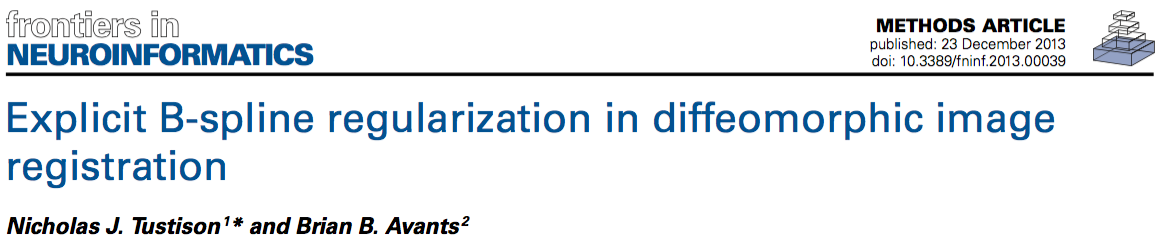
\includegraphics{./papers/figures/Frontiers_BSplineSyN.png}

\end{frame}

\begin{frame}{Template building: creating the average Joe}

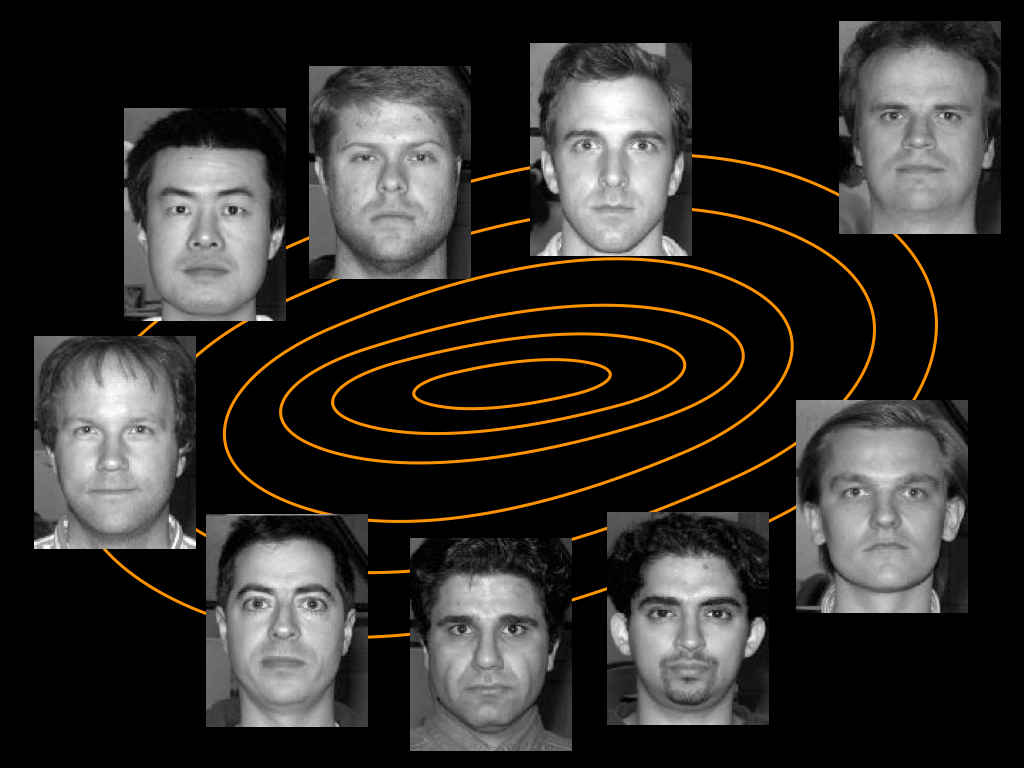
\includegraphics{./papers/figures/template0.jpg}

\end{frame}

\begin{frame}{``Attractiveness'' \(\rightarrow\) mental processing?}

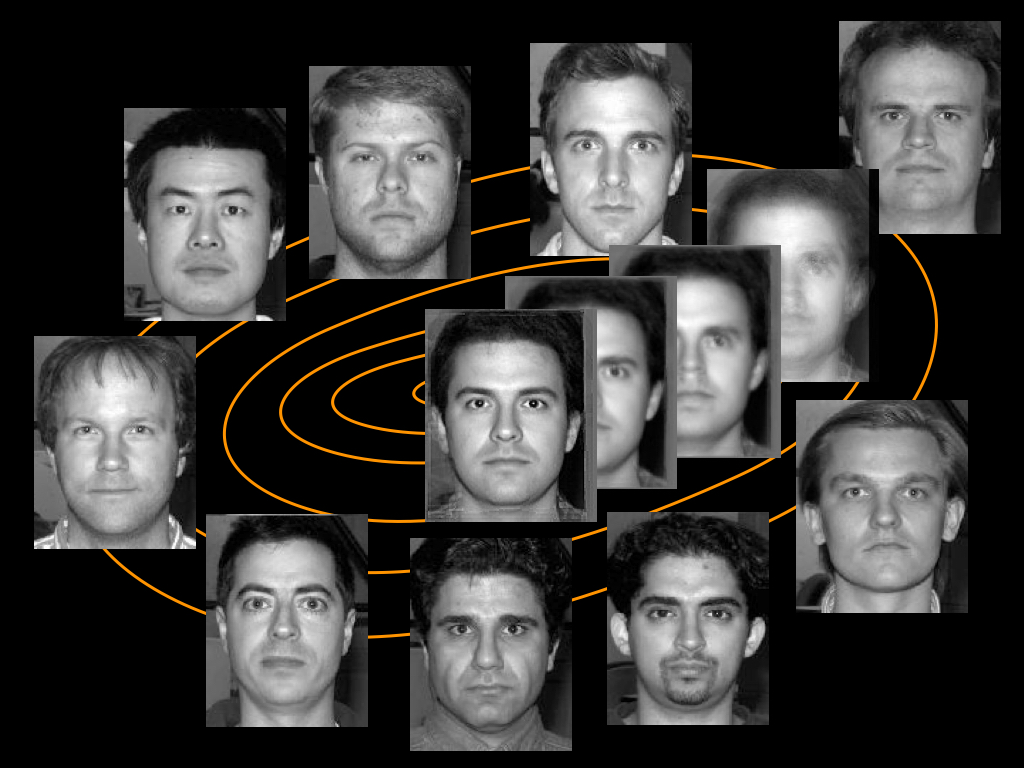
\includegraphics{./papers/figures/template1.jpg}

\end{frame}

\begin{frame}{What about brains?}

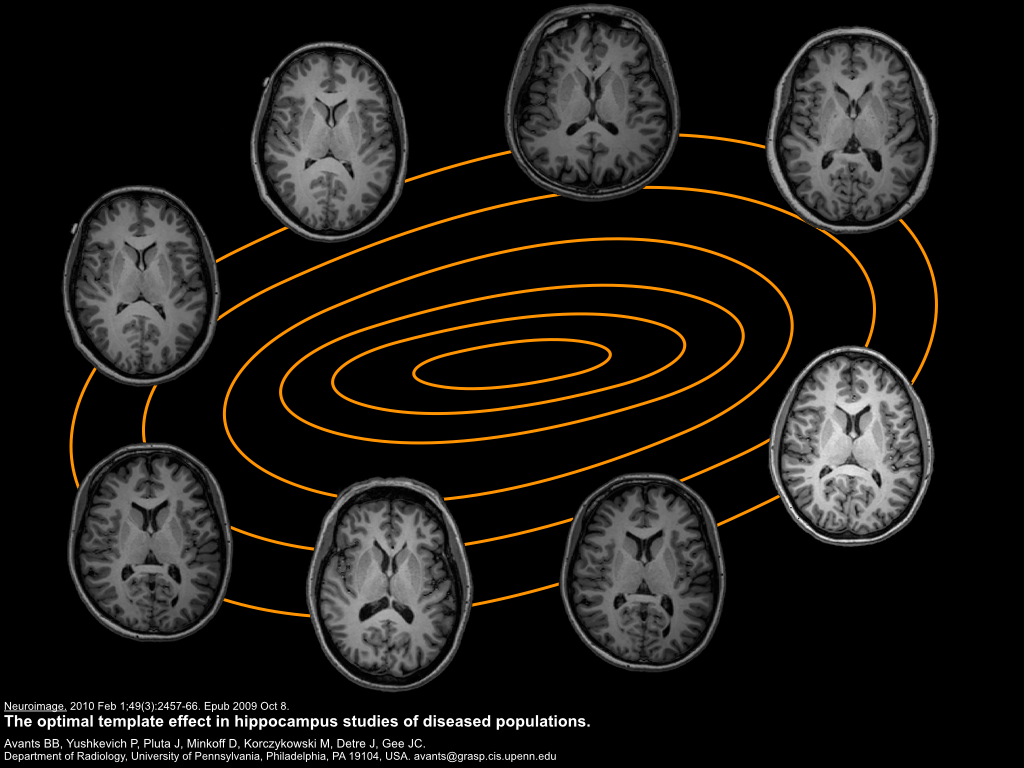
\includegraphics{./papers/figures/template3.jpg}

\end{frame}

\begin{frame}{Templates facilitate computation}

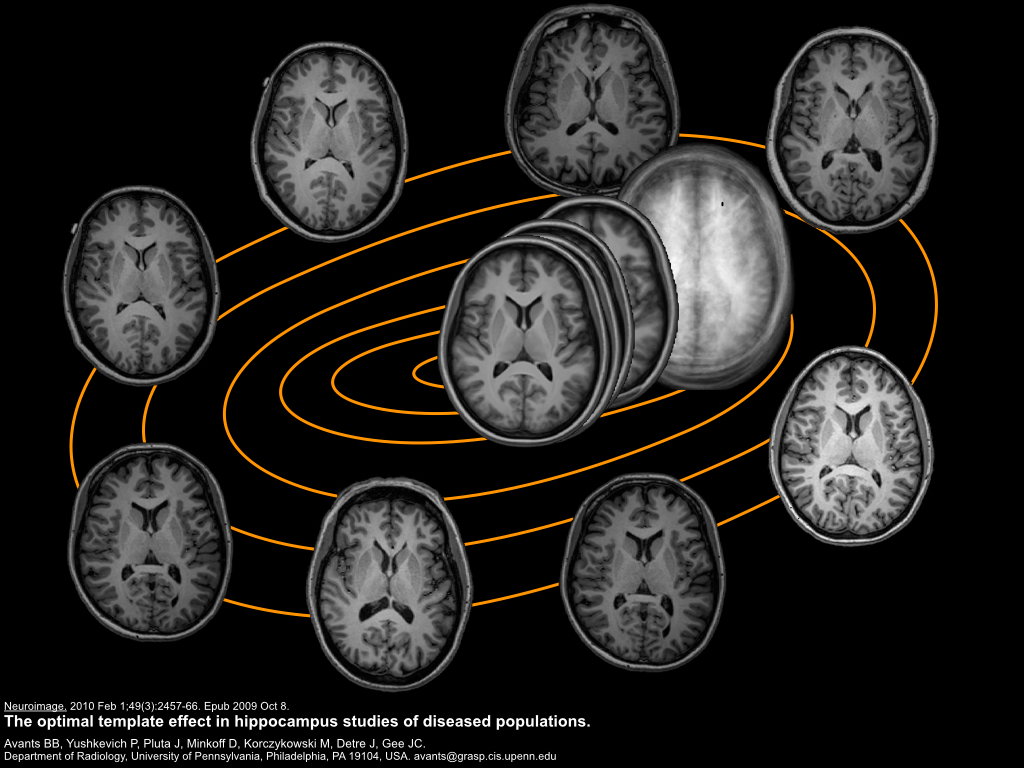
\includegraphics{./papers/figures/template4.jpg}

\end{frame}

\begin{frame}{Nonparametric nonuniform intensity normalization (N3)}

\begin{itemize}
\item
  Developed at the Montreal Neurological Institute (John Sled, 1998)
\item
  Part of the standard preprocessing protocol in large scale projects
  such as ADNI
\item
  The traditional de facto standard in MRI bias correction

  \begin{itemize}
  \tightlist
  \item
    good performance
  \item
    \emph{public availability}
  \end{itemize}
\item
  Public availability --- set of perl scripts coordinating various C++
  programs
\item
  ``\emph{Let's incorporate N3 into ANTs!}''
\end{itemize}

\end{frame}

\begin{frame}[fragile]{N4 (``Nick's N3'')}

\begin{itemize}
\item
  comparative
  \href{http://www.ncbi.nlm.nih.gov/pubmed/20378467}{evaluation}
\item
  small spline distances (useful for higher magnet strengths)
\item
  multiresolution
\item
  weighted regional mask (used in
  \href{https://github.com/stnava/ANTs/blob/master/Scripts/antsAtroposN4.sh}{\texttt{antsAtroposN4.sh}})
\item
  fast execution times
\item
  \emph{publicly available}
\item
  tested nightly within the ITK dashboard system
\end{itemize}

\end{frame}

\begin{frame}{Multi-atlas segmentation}

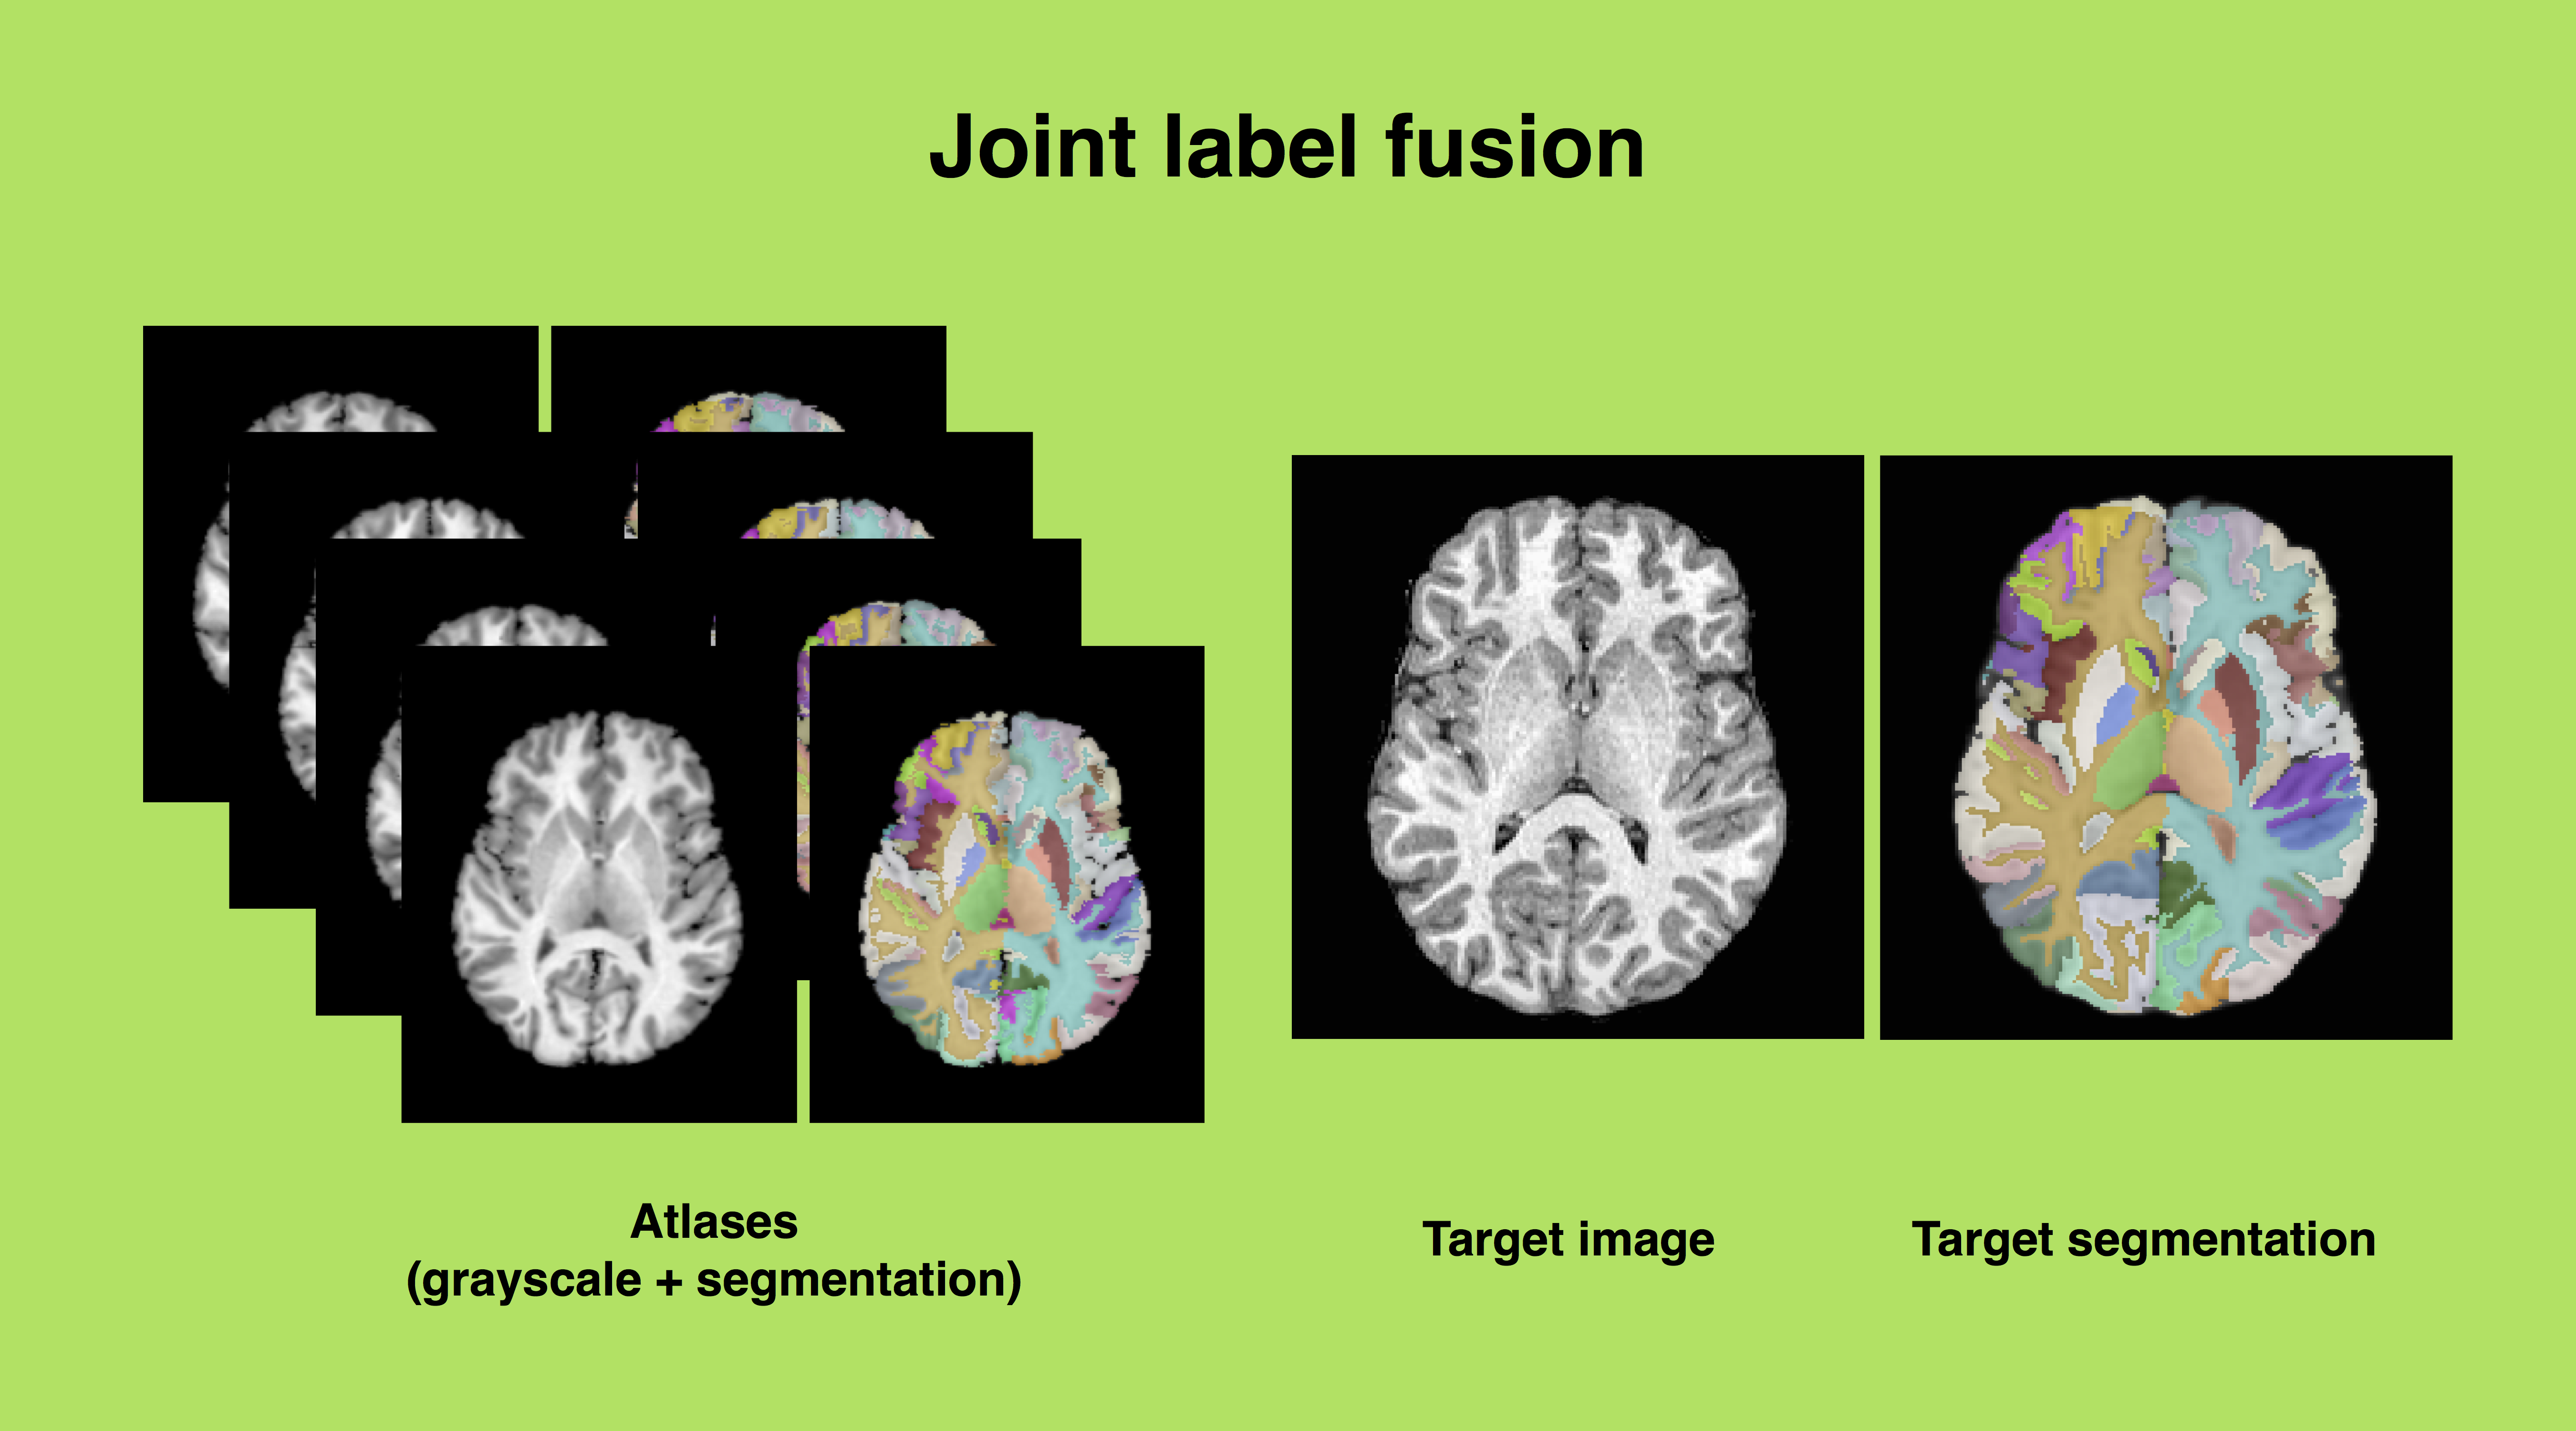
\includegraphics{./tools/jointfusion/figures/jointLabelFusion.png}

\end{frame}

\begin{frame}{New work: joint intensity fusion}

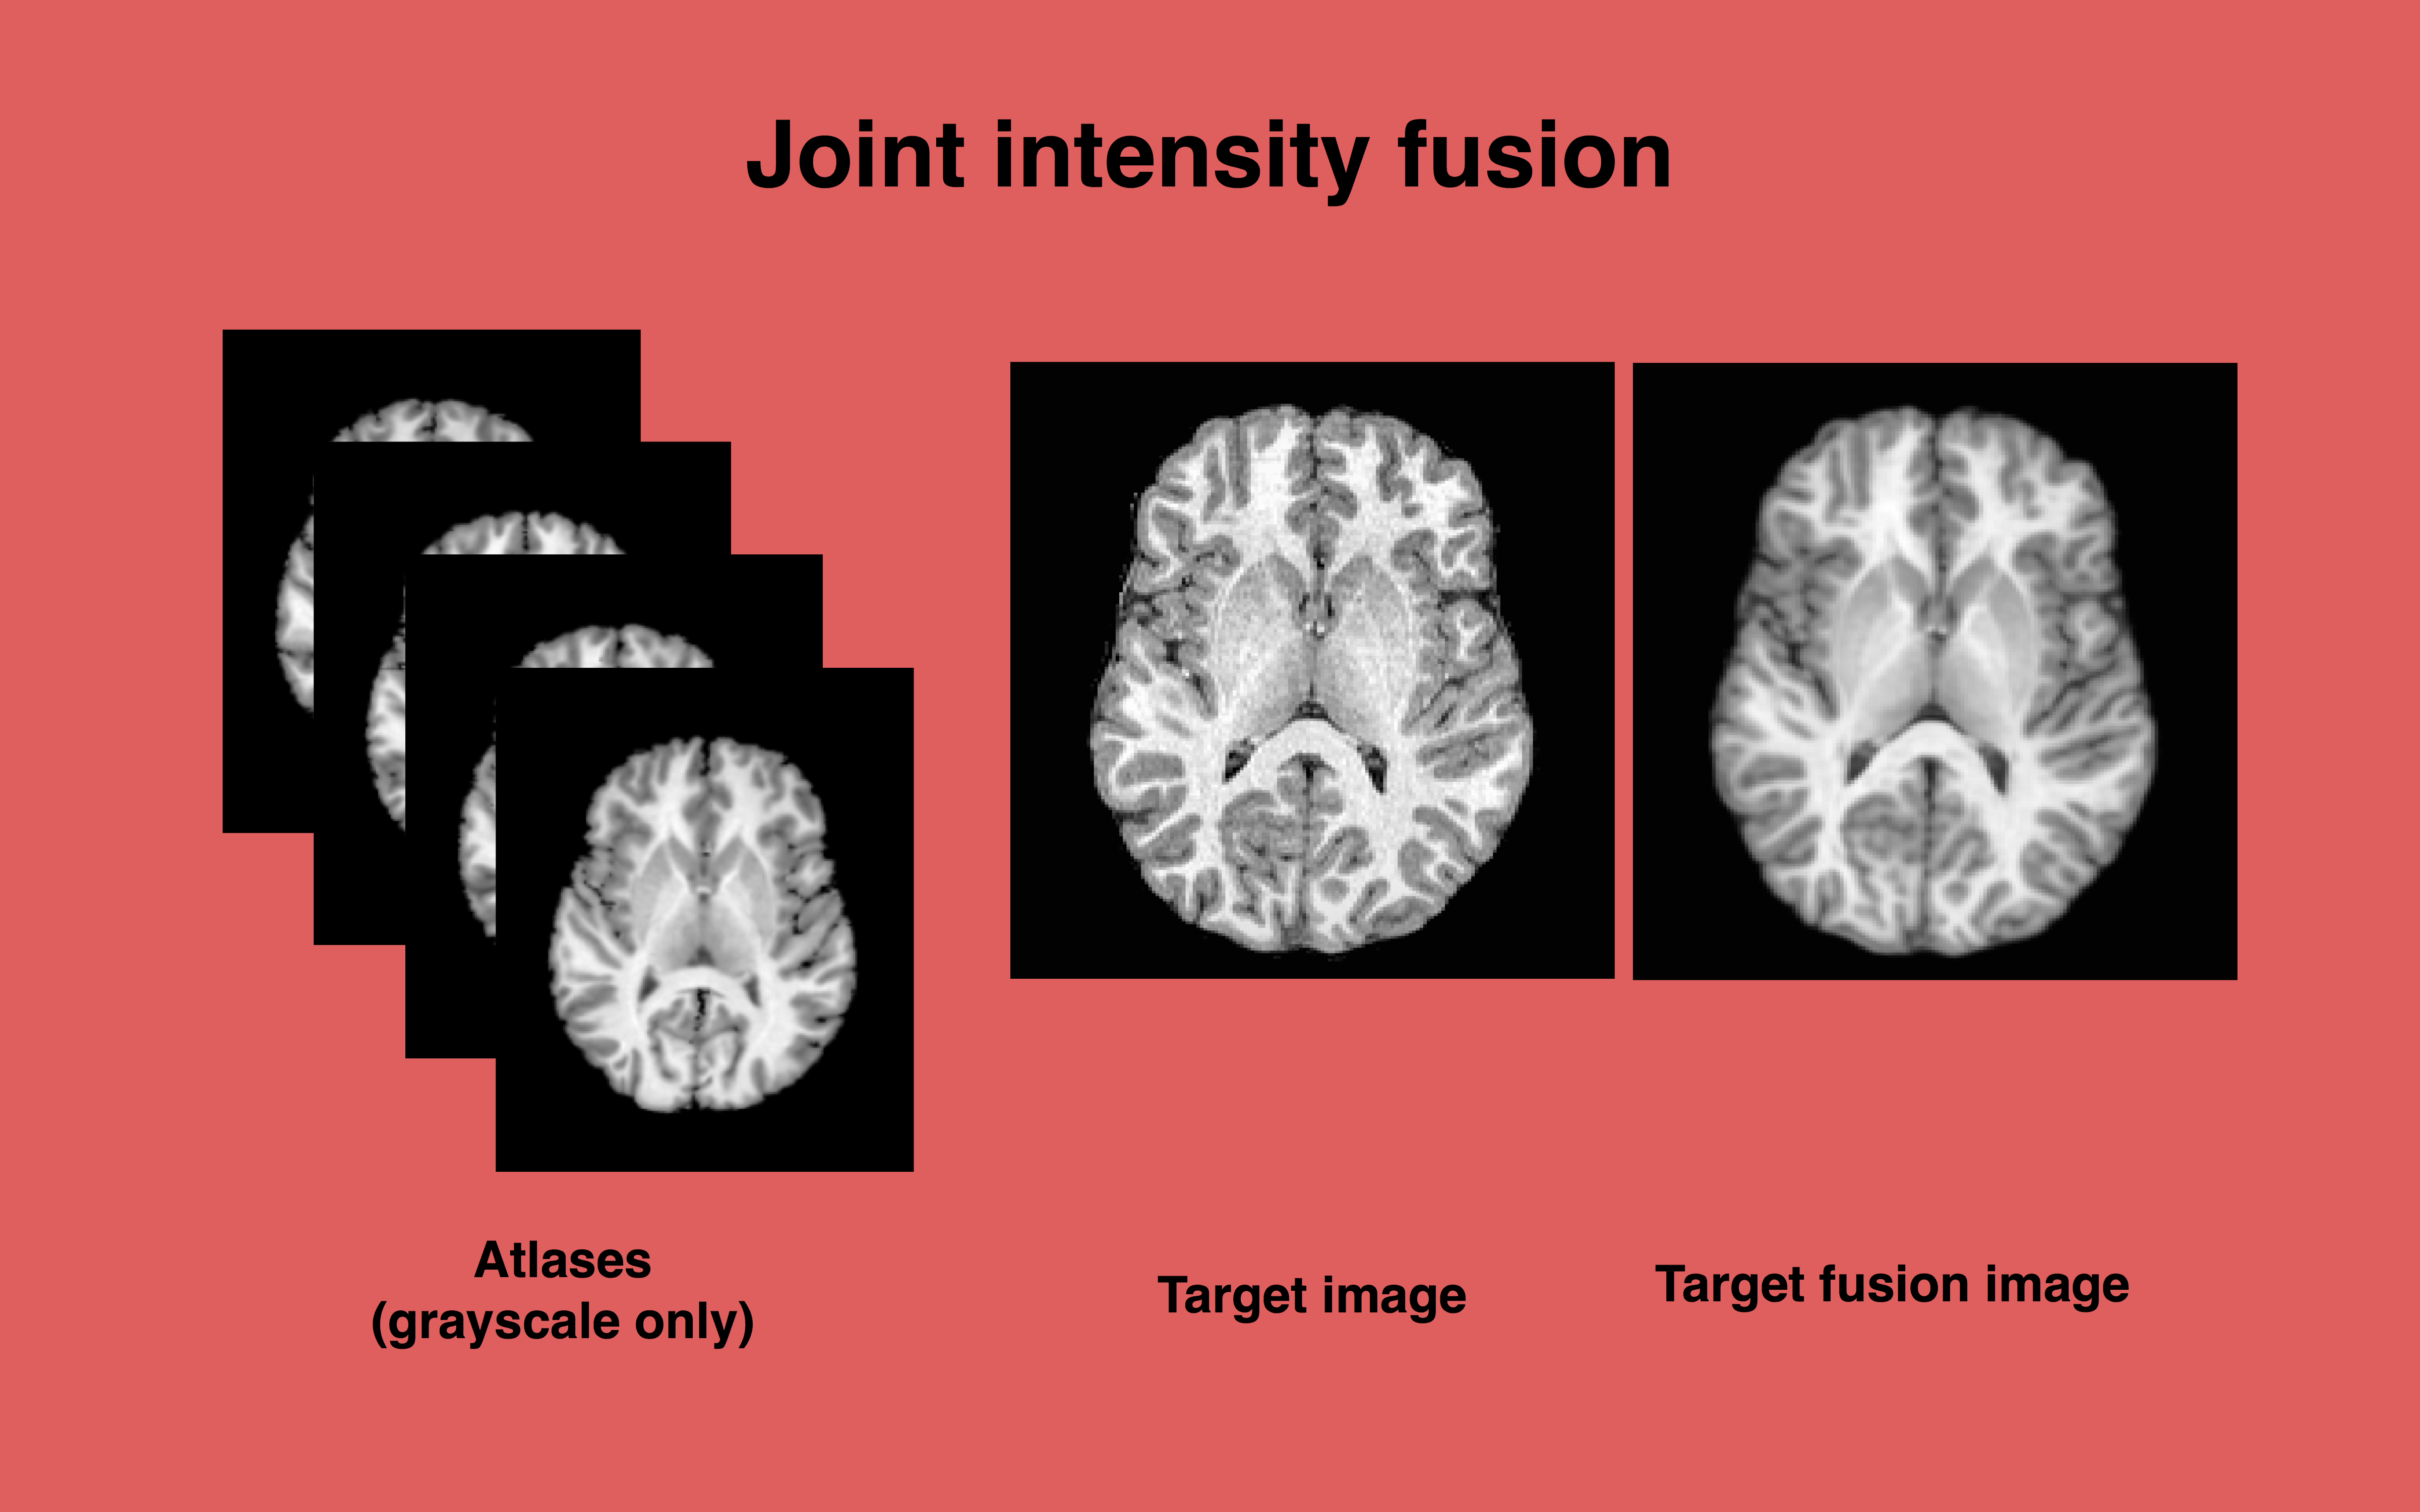
\includegraphics{./tools/jointfusion/figures/jointIntensityFusion.png}

\end{frame}

\begin{frame}{Possible uses}

\begin{itemize}
\item
  ``Correct'' images

  \begin{itemize}
  \item
    motion correction
  \item
    ``remove'' lesions
  \end{itemize}
\item
  Project atlas set intensity signature
\item
  Use in ``corrective learning''
\end{itemize}

\end{frame}

\section{Putting it all together---the ANTs cortical thickness
pipeline}\label{putting-it-all-togetherthe-ants-cortical-thickness-pipeline}

\begin{frame}{Cortical thickness studies}

\begin{longtable}[c]{@{}ll@{}}
\toprule
Column1 & Column2\tabularnewline
\midrule
\endhead
Tetris-playing ability & chronic pancreatitis\tabularnewline
Huntington's disease & obsessive-compulsive disorder\tabularnewline
schizophrenia & ADHD\tabularnewline
bipolar disorder & obesity\tabularnewline
Alzheimer's disease & heritable depression\tabularnewline
frontotemporal dementia & elderly depression\tabularnewline
Parkinson's disease & age\tabularnewline
Williams syndrome & gender\tabularnewline
multiple sclerosis & handedness\tabularnewline
autism & intelligence\tabularnewline
migraines & athletic ability\tabularnewline
chronic smoking & meditative practices\tabularnewline
alcoholism & musical ability\tabularnewline
cocaine addiction & tendency toward criminality\tabularnewline
Tourette syndrome in children & childhood sexual abuse in female
adolescents\tabularnewline
scoliosis in female adolescents & traumatic brain injury\tabularnewline
early-onset blindness & untreated male-to-female
transsexuality\tabularnewline
\bottomrule
\end{longtable}

\end{frame}

\begin{frame}{The ANTs structural brain mapping workflow}

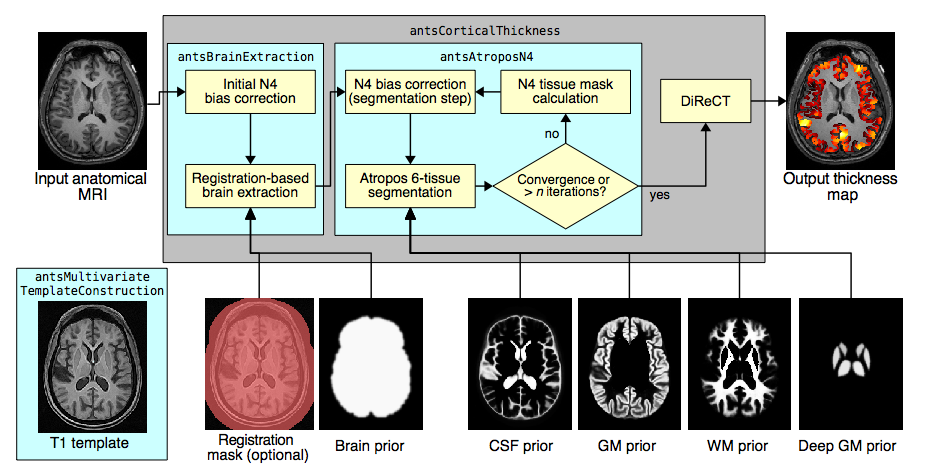
\includegraphics{./evaluation/figures/pipeline.png}

\end{frame}

\begin{frame}{Template building}

\emph{Tailor data to your specific cohort}

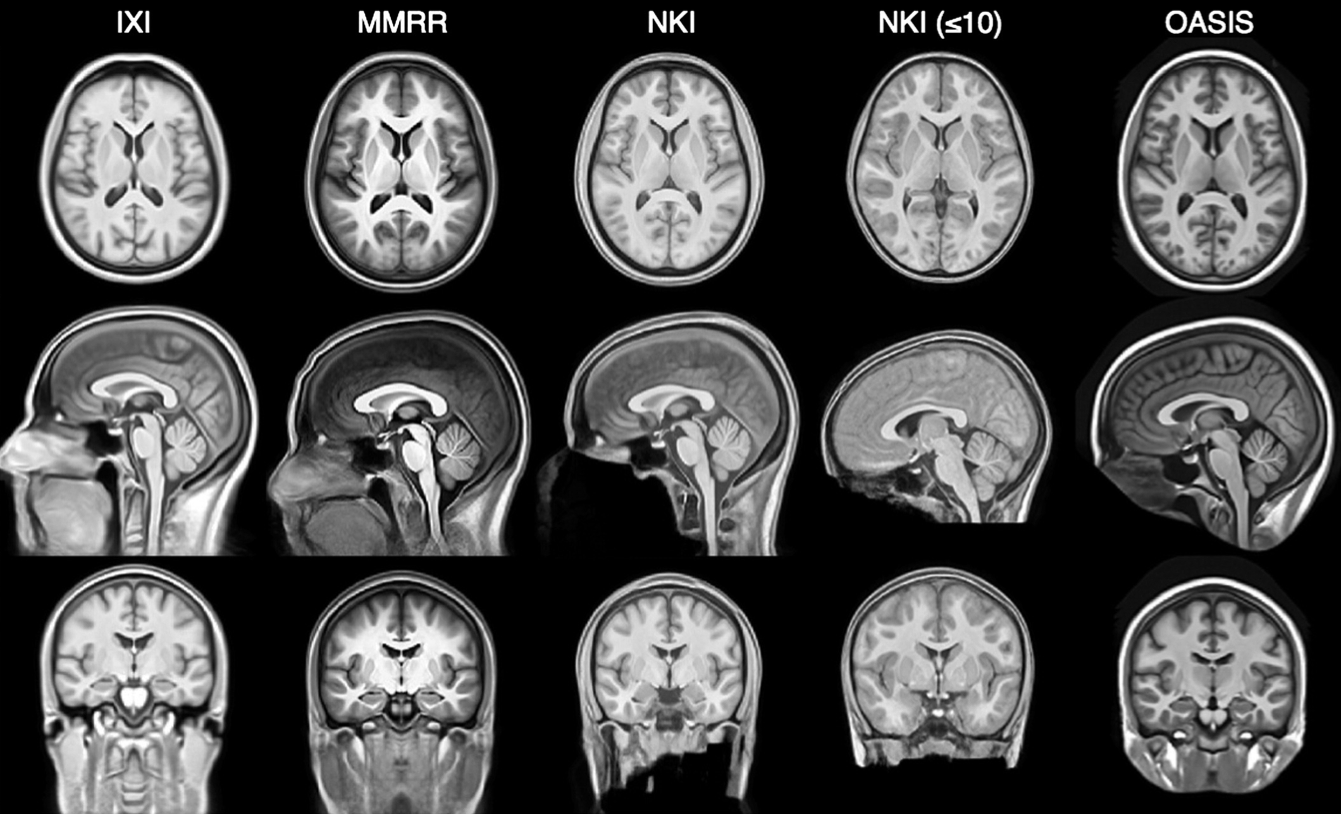
\includegraphics{./evaluation/figures/templates.png}

\end{frame}

\begin{frame}{Template priors}

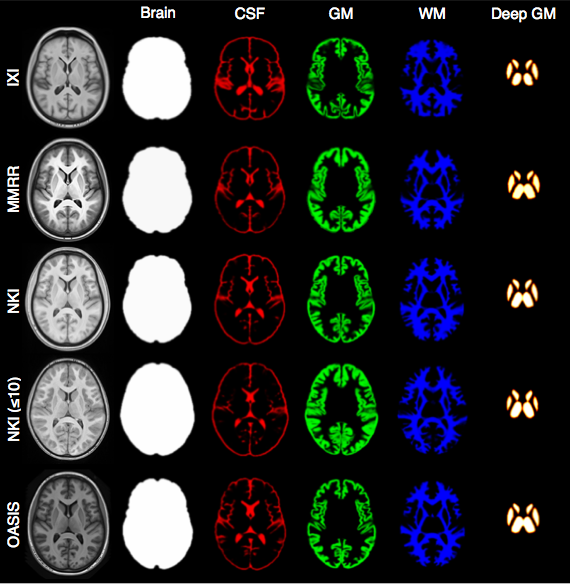
\includegraphics{./evaluation/figures/templatePriors.png}

\end{frame}

\begin{frame}{Cortical thickness maps}

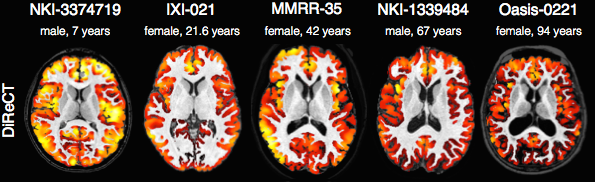
\includegraphics{./evaluation/figures/corticalThicknessEstimation.png}

In contrast to FreeSurfer which warps coupled surface meshes to segment
the gray matter, \emph{ANTs} diffeomorphically registers the white
matter to the combined gray/white matters while simultaneously
estimating thickness.

\end{frame}

\begin{frame}

\emph{But without ground truth, how does one evaluate the pipeline?}

\end{frame}

\begin{frame}{Predict age and gender}

\(AGE \sim VOLUME + GENDER + \sum_{i=1}^{62} T(DKT_i)\)

\end{frame}

\begin{frame}{Prediction from cortical thickness data}

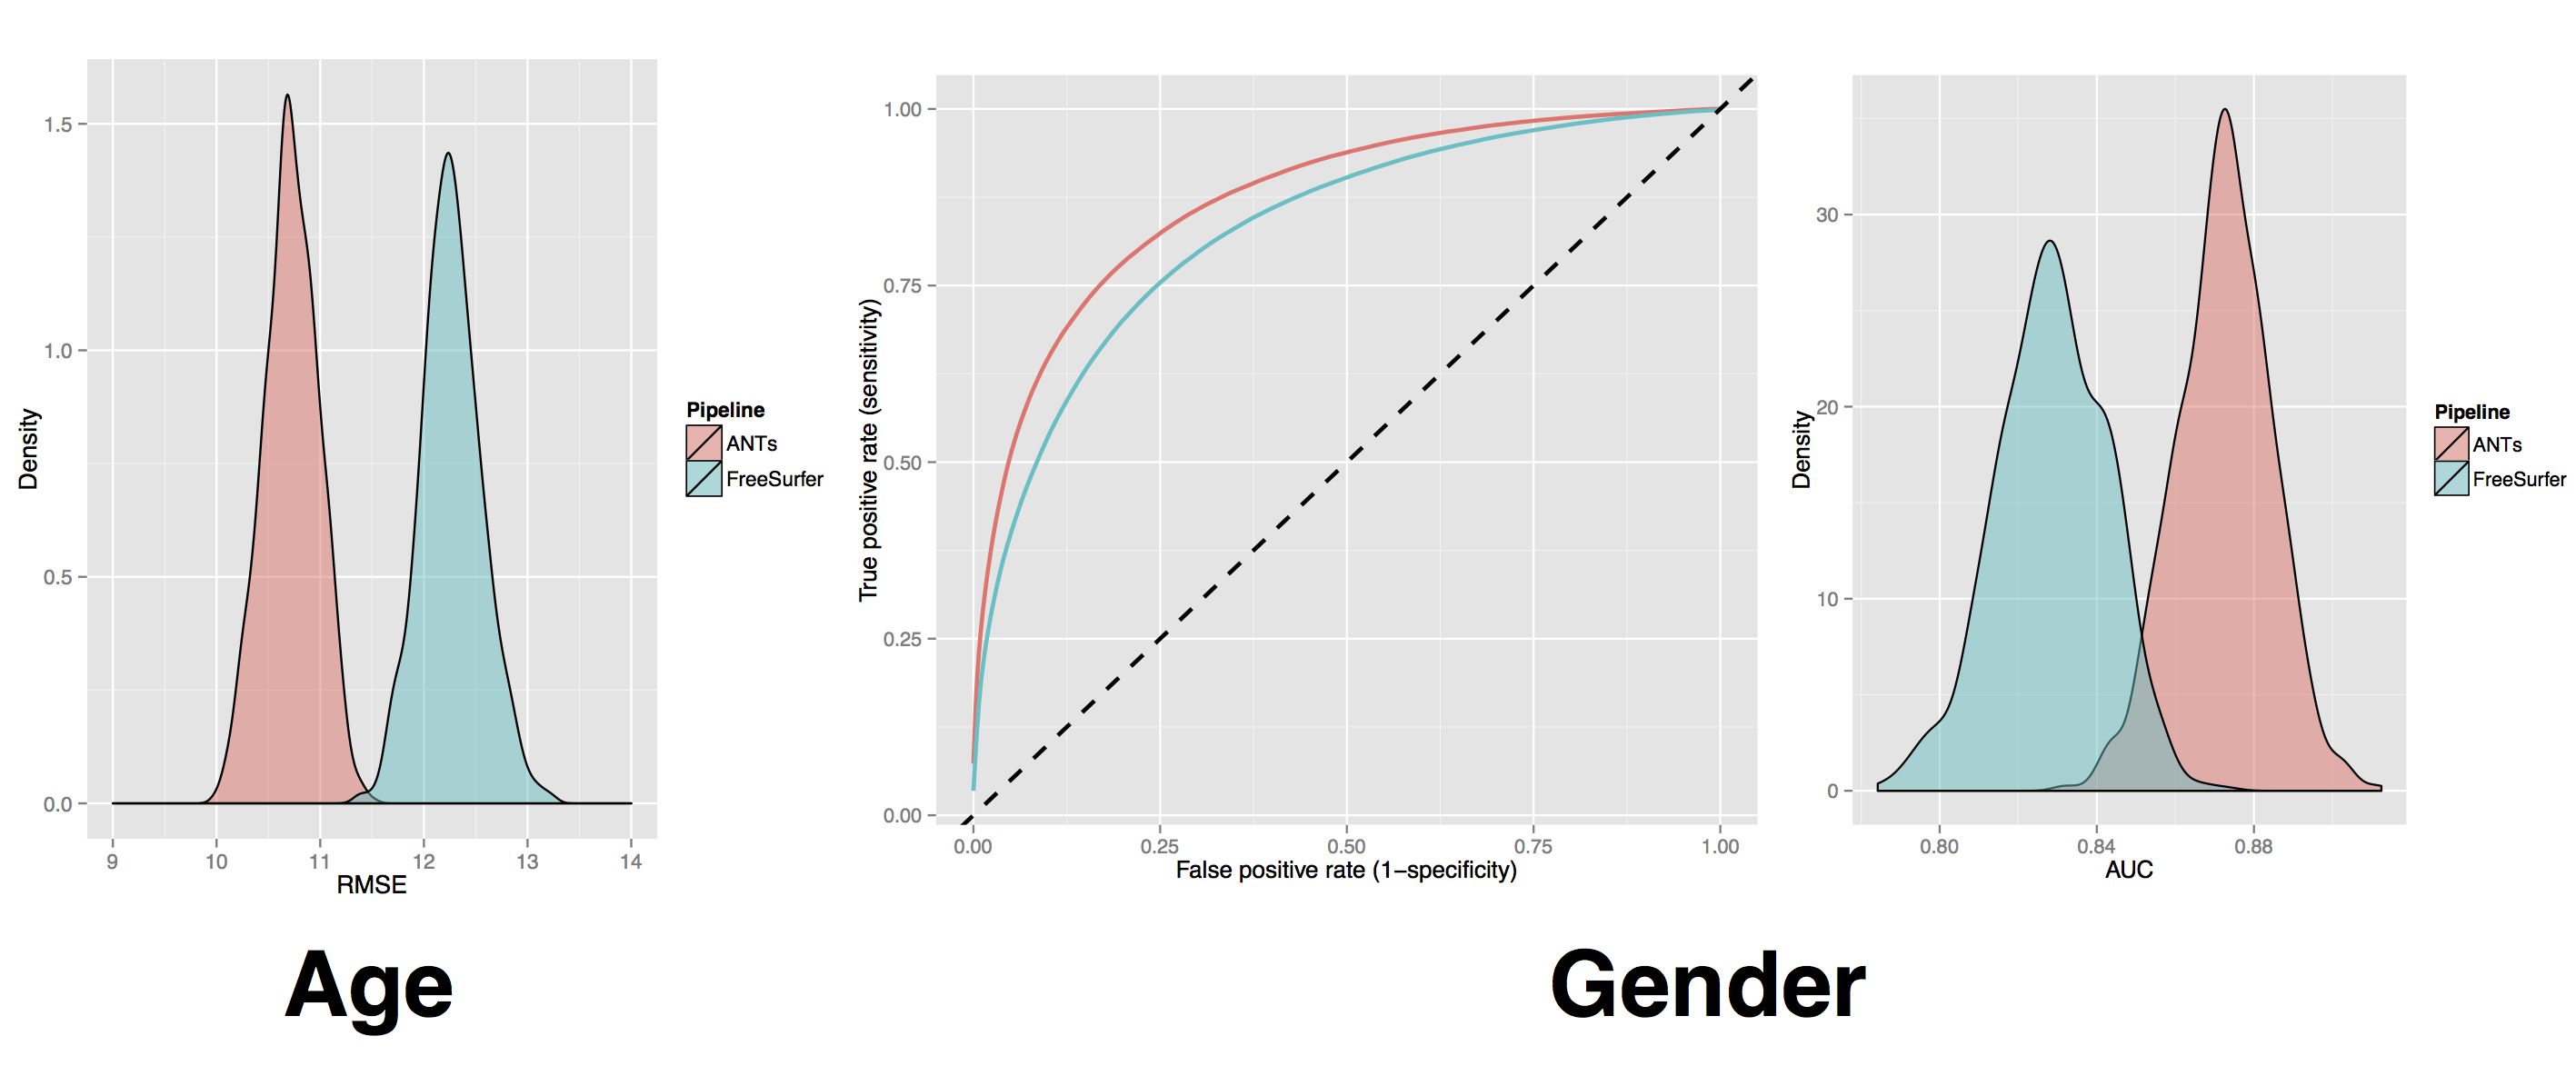
\includegraphics{./evaluation/figures/evaluation.png}

\end{frame}

\section{Current work and Advanced Normalization Tools in R
(ANTsR)}\label{current-work-and-advanced-normalization-tools-in-r-antsr}

\begin{frame}{Multimodal Brain Tumor Segmentation (BRATS 2013)}

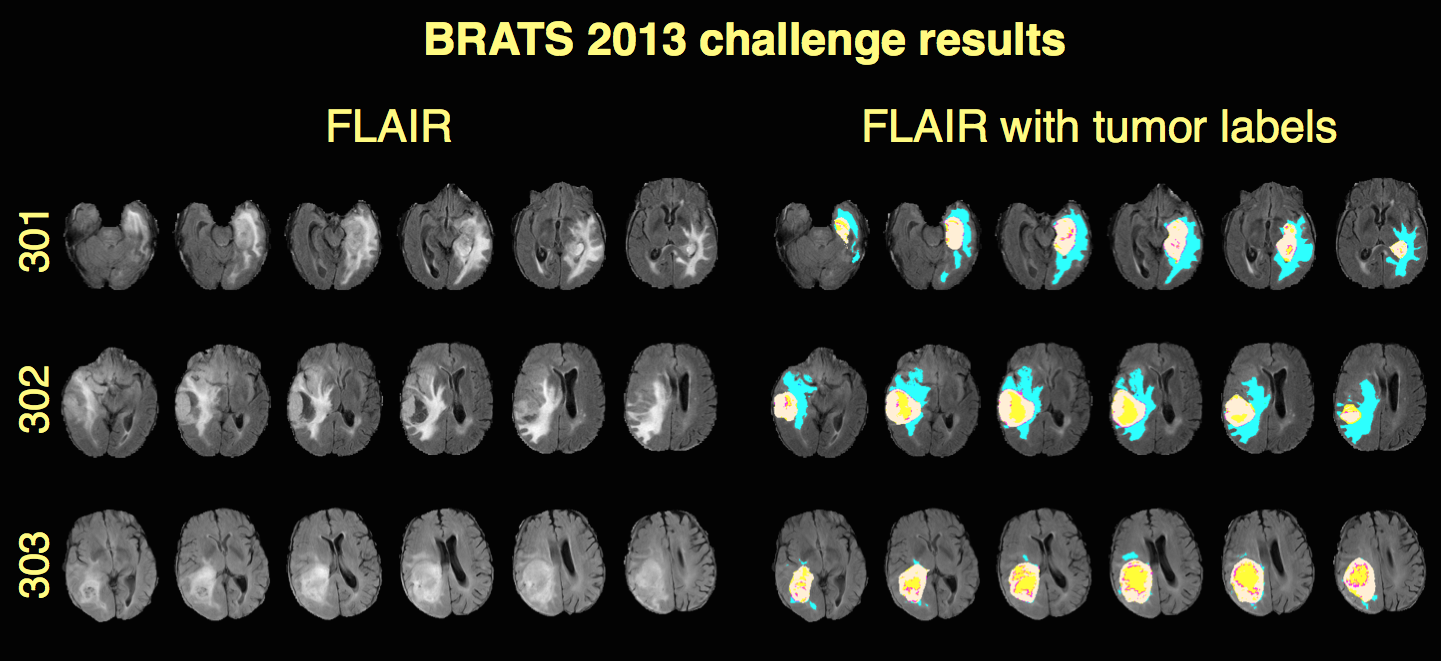
\includegraphics{./competitions/figures/brats2013results1.png}

\href{http://www.ncbi.nlm.nih.gov/pubmed/25433513}{Tustison, et al.,
Optimal symmetric multimodal templates and concatenated random forests
for supervised brain tumor segmentation (simplified) with \emph{ANTsR},
\emph{Neuroinformatics}.}

\end{frame}

\begin{frame}{White matter hyperintensities in TBI}

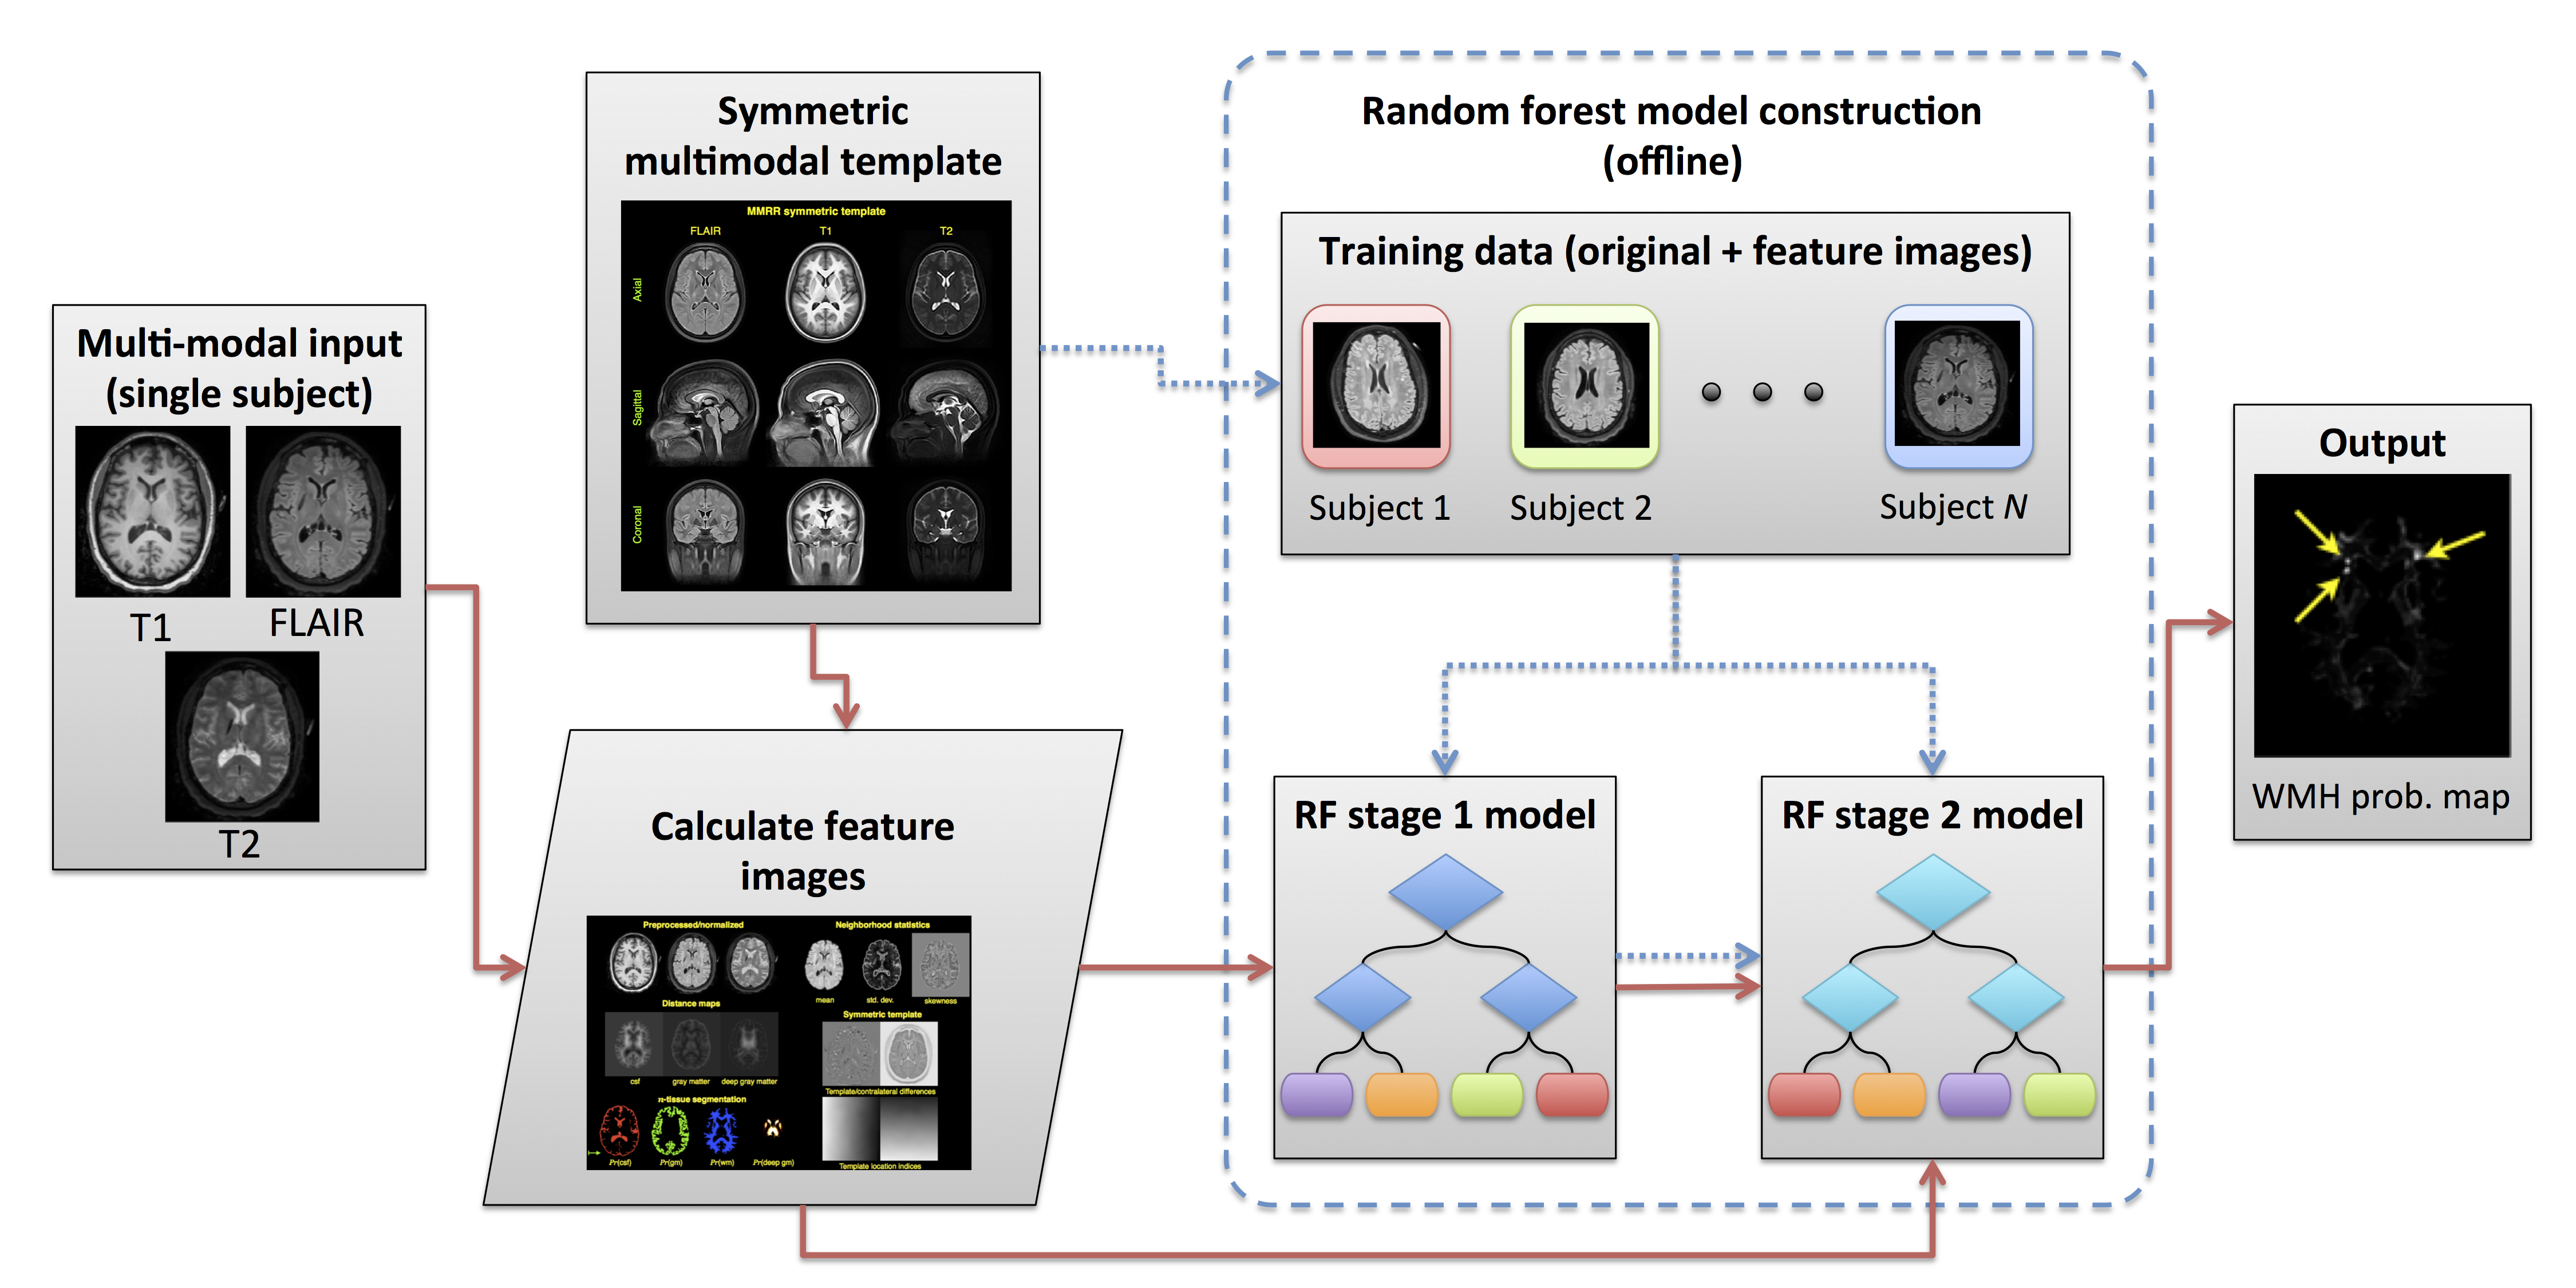
\includegraphics{./wmhs/figures/wmhPipeline.png}

\end{frame}

\begin{frame}{Social behavior and immunity dysfunction in mice}

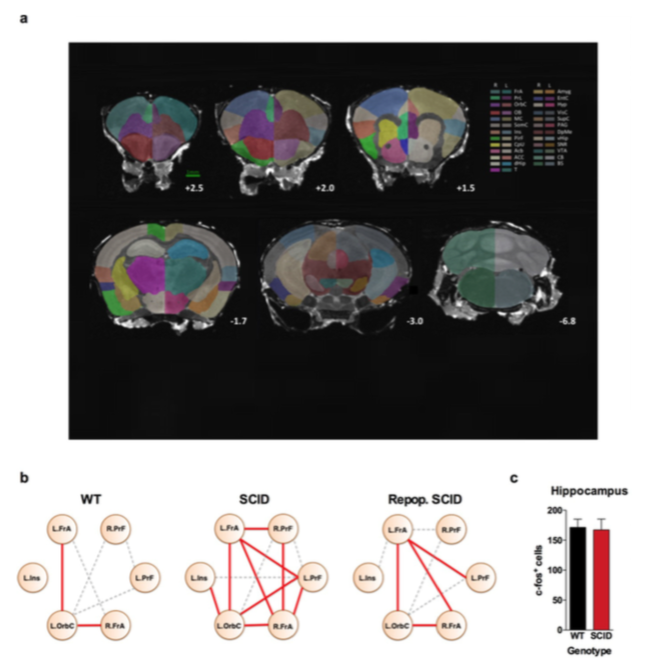
\includegraphics{./antsr/figures/filiano_rsfmri.png}

\hypertarget{refs}{}

\end{frame}

\end{document}
